\documentclass[11pt]{article}
\usepackage[margin=1in]{geometry}
\usepackage{amsmath,amssymb,amsthm}
\usepackage{graphicx,float}
\usepackage{lmodern}
\usepackage[T1]{fontenc}
\usepackage{xcolor,framed,booktabs,microtype,array}
\usepackage[colorlinks=true,linkcolor=blue!60!black,urlcolor=blue!60!black]{hyperref}

\definecolor{shadecolor}{RGB}{240,244,250}
\definecolor{warncolor}{RGB}{253,242,235}
\newenvironment{keyidea}{\begin{shaded}\noindent\textbf{Key idea.} }{\end{shaded}}
\newenvironment{pitfall}{\colorlet{shadecolor}{warncolor}\begin{shaded}\noindent\textbf{Common pitfall.} }{\end{shaded}}
\newenvironment{template}{\begin{framed}\noindent\textbf{Proof template.} }{\end{framed}}

\newcommand{\R}{\mathbb{R}}
\newcommand{\norm}[1]{\left\lVert #1 \right\rVert}
\newcommand{\T}{^{\mathsf T}}
\newcommand{\lam}{\lambda}
\newcommand{\epi}{\operatorname{epi}}
\newcommand{\dom}{\operatorname{dom}}
\newcommand{\conv}{\operatorname{conv}}

\theoremstyle{definition}
\newtheorem{definition}{Definition}[section]
\theoremstyle{plain}
\newtheorem{theorem}[definition]{Theorem}
\newtheorem{proposition}[definition]{Proposition}
\theoremstyle{remark}
\newtheorem{example}[definition]{Example}
\newtheorem{exercise}[definition]{Self-test}

\title{Convex Sets, Convex Functions, and Hyperplanes\\ \large A study guide for the material of Homework 1}
\author{Optimization (Caramanis \& Sanghavi) --- companion notes}
\date{\today}

\begin{document}
\maketitle

\tableofcontents
\bigskip

\section{Why convexity is the whole game}

An optimization problem $\min_{x\in\mathcal F} f(x)$ is \emph{convex} when the feasible set $\mathcal F$ is a convex set and the objective $f$ is a convex function. Two facts make this class special:
\begin{enumerate}
\item \textbf{Local = global.} Every local minimizer of a convex problem is a global minimizer. Descent methods therefore cannot get ``stuck.''
\item \textbf{Certifiable optimality.} There is a clean first-order optimality condition ($\nabla f(x^\star)\T(y-x^\star)\ge0$ for all feasible $y$) and a duality theory that produces \emph{proofs} of optimality.
\end{enumerate}
Everything in this unit is machinery for recognising, building, and manipulating convex sets and functions. The homework tests three skills that recur all semester:
\begin{itemize}
\item proving a set or function is convex \emph{from the definition};
\item knowing which \emph{operations preserve} convexity (and which do not);
\item translating geometric statements (``closer to $v_1$ than $v_2$'') into algebraic ones (``$c\T x\le d$'').
\end{itemize}

\section{Convex sets}

\subsection{Definitions}

\begin{definition}[Convex set]
$C\subseteq\R^n$ is \emph{convex} if for all $x,y\in C$ and all $\lam\in[0,1]$, $\;\lam x+(1-\lam)y\in C$.
\end{definition}
The point $\lam x+(1-\lam)y$ traces the closed segment from $y$ ($\lam=0$) to $x$ ($\lam=1$). So ``convex'' means: \emph{the segment joining any two points of the set stays in the set}. The empty set, a single point, and all of $\R^n$ are convex.

\begin{figure}[H]\centering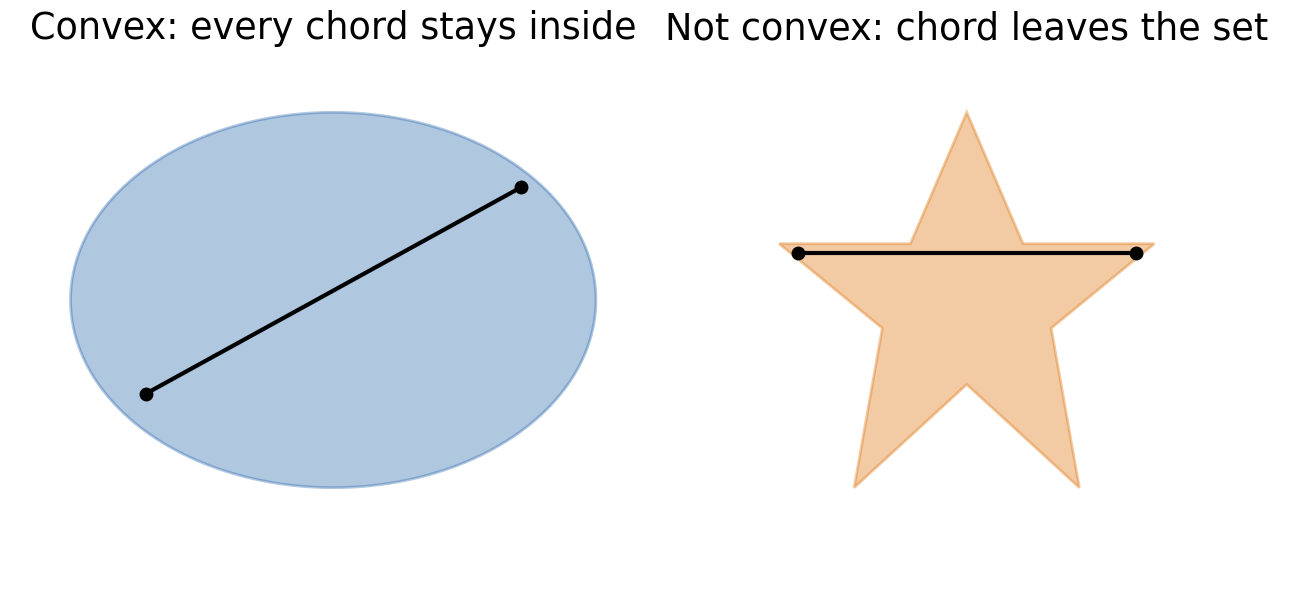
\includegraphics[width=.75\textwidth]{figures/convex_vs_nonconvex.png}\end{figure}

\begin{definition}[Related notions]\leavevmode
\begin{itemize}
\item A \emph{convex combination} of $x_1,\dots,x_k$ is $\sum_i\theta_ix_i$ with $\theta_i\ge0$, $\sum_i\theta_i=1$. A set is convex iff it is closed under all convex combinations (induction on $k$).
\item The \emph{convex hull} $\conv S$ is the set of all convex combinations of points of $S$; it is the smallest convex set containing $S$.
\item $C$ is \emph{affine} if it contains the whole \emph{line} through any two of its points ($\lam\in\R$). Affine $\Rightarrow$ convex.
\item $C$ is a \emph{cone} if $x\in C,\ \theta\ge0\Rightarrow\theta x\in C$; a \emph{convex cone} is closed under all conic combinations $\theta_1x_1+\theta_2x_2$, $\theta_i\ge0$.
\end{itemize}
\end{definition}

\subsection{The examples you must know}
\begin{center}\begin{tabular}{@{}lll@{}}\toprule
Set & Formula & Why convex \\ \midrule
Hyperplane & $\{x:a\T x=b\}$, $a\ne0$ & affine \\
Half-space & $\{x:a\T x\le b\}$, $a\ne0$ & linear inequality survives averaging \\
Euclidean ball & $\{x:\|x-x_c\|_2\le r\}$ & triangle inequality \\
Norm ball & $\{x:\|x-x_c\|\le r\}$, any norm & triangle inequality \\
Ellipsoid & $\{x:(x-x_c)\T P^{-1}(x-x_c)\le1\}$, $P\succ0$ & image of ball under $P^{1/2}$ \\
Norm cone & $\{(x,t):\|x\|\le t\}$ & sublevel set of convex $\|x\|-t$ \\
Polyhedron & $\{x:Ax\preceq b,\ Cx=d\}$ & intersection of half-spaces/hyperplanes \\
Simplex & $\conv\{v_0,\dots,v_k\}$ & convex hull \\
PSD cone $\mathbb S^n_+$ & $\{X=X\T:X\succeq0\}$ & $z\T(\lam X+(1-\lam)Y)z\ge0$ \\
Voronoi cell of $v_1$ & $\{x:\|x-v_1\|\le\|x-v_j\|\ \forall j\}$ & intersection of half-spaces (HW1 P3) \\ \bottomrule
\end{tabular}\end{center}

\subsection{Operations that preserve convexity of sets}
\begin{theorem}[Calculus of convex sets]\label{thm:setcalc}\leavevmode
\begin{enumerate}
\item \textbf{Intersection.} If $C_\alpha$ is convex for every $\alpha$ in an arbitrary index set, then $\bigcap_\alpha C_\alpha$ is convex. \emph{(HW1 P1a.)}
\item \textbf{Affine image and preimage.} If $f(x)=Ax+b$ is affine, $C$ convex $\Rightarrow f(C)$ convex, and $D$ convex $\Rightarrow f^{-1}(D)=\{x:Ax+b\in D\}$ convex. Special cases: scaling, translation, projection onto coordinates, Minkowski sum $C_1+C_2$, Cartesian product $C_1\times C_2$.
\item \textbf{Perspective and linear-fractional maps} also preserve convexity (B\&V \S2.3.3); rarely tested at this stage.
\end{enumerate}
\end{theorem}

\begin{proof}[Proof of 1]
Take $x,y\in\bigcap_\alpha C_\alpha$, $\lam\in[0,1]$. For each $\alpha$, $x,y\in C_\alpha$ and $C_\alpha$ convex give $\lam x+(1-\lam)y\in C_\alpha$. True for every $\alpha$, hence true for the intersection.
\end{proof}
\begin{proof}[Proof of 2 (preimage)]
If $Ax+b\in D$ and $Ay+b\in D$, then $A(\lam x+(1-\lam)y)+b=\lam(Ax+b)+(1-\lam)(Ay+b)\in D$ by convexity of $D$. The image case is similar.
\end{proof}

\begin{pitfall}
\textbf{Unions and complements do not preserve convexity.} $[0,1]\cup[2,3]$ is not convex; the complement of a disk is not convex. When you see ``union'' or ``or'' in a set description, expect non-convexity unless the pieces overlap heavily. \emph{(HW1 P1b.)}
\end{pitfall}

\begin{keyidea}
To prove a complicated set is convex, \emph{do not} start from the definition. Instead, write it as (i) an intersection of simpler convex sets, or (ii) an affine preimage of a standard convex set, or (iii) a sublevel set of a convex function. Example: $\{x:\|Ax+b\|_2\le c\T x+d\}$ is the preimage of the second-order cone under the affine map $x\mapsto(Ax+b,\,c\T x+d)$. \emph{(HW1 P4.)}
\end{keyidea}

\section{Hyperplanes and half-spaces}

\subsection{Geometry of $a\T x=b$}
Fix $a\ne0$. The hyperplane $H=\{x:a\T x=b\}$ is the set of $x$ with a fixed inner product with $a$. Equivalently, picking any $x_0\in H$, $H=\{x:a\T(x-x_0)=0\}=x_0+a^\perp$: it is the translate of the $(n-1)$-dimensional subspace orthogonal to $a$. The vector $a$ is the \emph{normal}; it points into the half-space $\{a\T x\ge b\}$ and away from $\{a\T x\le b\}$.

\begin{proposition}[Distance formulas]\leavevmode
\begin{enumerate}
\item Distance from a point $x$ to $H=\{a\T x=b\}$: $\ \operatorname{dist}(x,H)=\dfrac{|a\T x-b|}{\|a\|_2}$. The closest point is $x-\dfrac{a\T x-b}{\|a\|^2}a$.
\item Distance between parallel hyperplanes $\{a\T x=b_1\}$, $\{a\T x=b_2\}$: $\ \dfrac{|b_1-b_2|}{\|a\|_2}$. \emph{(HW1 P5b.)}
\end{enumerate}
\end{proposition}
\emph{Mnemonic:} normalise $a$ to a unit vector; then $b$ is the signed offset of the plane along $a$.

\begin{figure}[H]\centering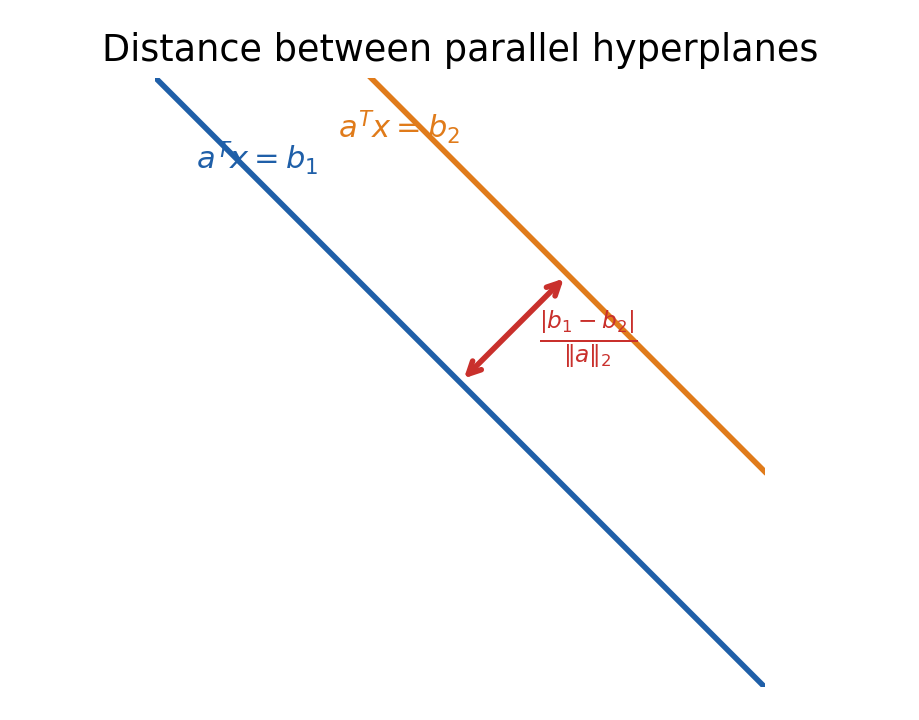
\includegraphics[width=.4\textwidth]{figures/parallel_hyperplanes.png}\end{figure}

\subsection{Containment and equality of half-spaces}
\begin{proposition}[B\&V 2.6, HW1 P5a]
For $a,\tilde a\ne0$:
\[
\{a\T x\le b\}\subseteq\{\tilde a\T x\le\tilde b\}\iff \tilde a=\lam a\text{ and }\tilde b\ge\lam b\text{ for some }\lam>0,
\]
with equality of the half-spaces iff additionally $\tilde b=\lam b$.
\end{proposition}
The proof strategy is instructive: assume containment, then \emph{walk to infinity} inside the small half-space along a direction $w\perp a$ (to show $\tilde a\parallel a$) and along $-a$ (to show the multiple is positive). Any direction in which the small half-space is unbounded must also leave the big one unbounded.

\subsection{Half-spaces from distance comparisons}
\begin{proposition}[Perpendicular bisector, HW1 P3]
For $v_1\ne v_2\in\R^n$,
\[
\{x:\|x-v_1\|_2\le\|x-v_2\|_2\}=\{x:c\T x\le d\},\qquad c=2(v_2-v_1),\quad d=\|v_2\|^2-\|v_1\|^2 .
\]
\end{proposition}
\begin{proof}[Idea]
Square both sides (allowed: both are $\ge0$), expand $\|x-v\|^2=\|x\|^2-2v\T x+\|v\|^2$, and watch the quadratic term $\|x\|^2$ cancel. What remains is linear in $x$.
\end{proof}
The boundary passes through the midpoint $\tfrac12(v_1+v_2)$ with normal $v_2-v_1$: it is the perpendicular bisector. Intersecting over many $v_j$ gives the Voronoi cell, convex by Theorem~\ref{thm:setcalc}(1).

\begin{figure}[H]\centering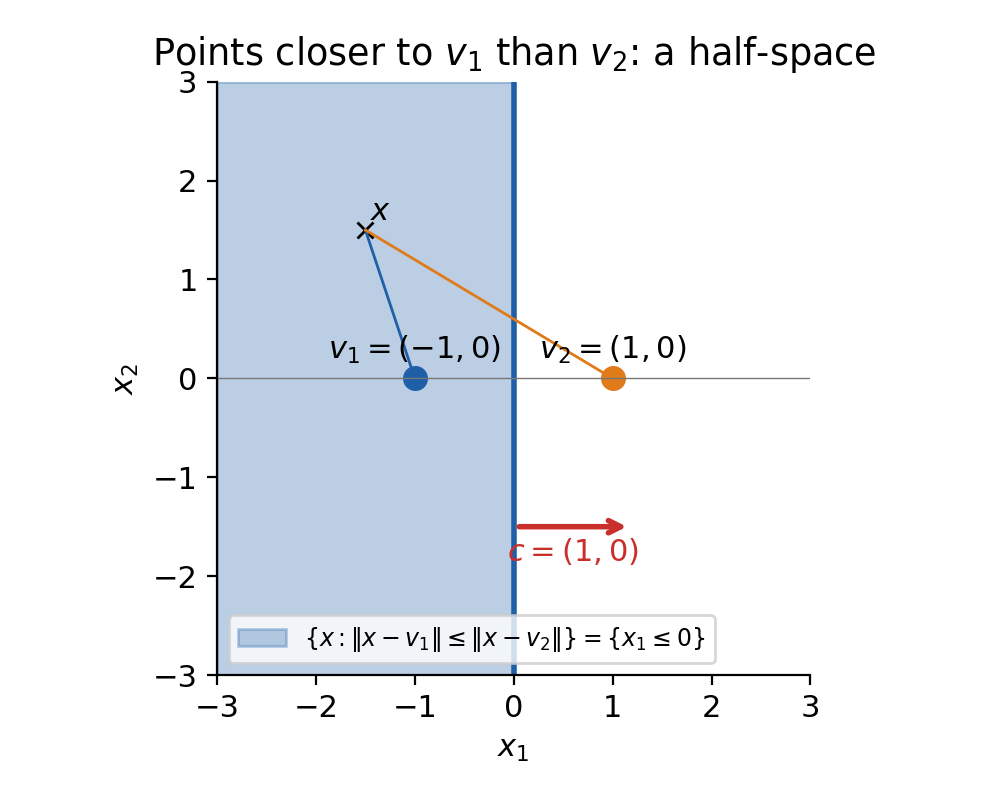
\includegraphics[width=.42\textwidth]{figures/halfspace_voronoi.png}\end{figure}

\begin{pitfall}
Sign and direction of $c$. The normal $c=2(v_2-v_1)$ points from $v_1$ \emph{toward} $v_2$, and the inequality is $c\T x\le d$. It is easy to flip a sign; always sanity-check with $x=v_1$ (must satisfy the inequality) and $x=v_2$ (must violate it unless $v_1=v_2$). Also, $c$ and $d$ are only defined up to a common positive factor.
\end{pitfall}

\section{Separating and supporting hyperplanes}

\begin{definition}
Hyperplane $\{a\T x=b\}$ ($a\ne0$) \emph{separates} $C$ and $D$ if $a\T x\le b$ on $C$ and $a\T x\ge b$ on $D$. It \emph{strictly separates} them if both inequalities are strict.
\end{definition}

\begin{theorem}[Separating hyperplane theorem]
If $C,D\subseteq\R^n$ are nonempty, convex, and disjoint, there exists a separating hyperplane.
\end{theorem}
\begin{theorem}[Strict separation]
If in addition $C$ is \textbf{closed} and $D$ is \textbf{compact} (closed and bounded), the separation can be taken strict; in fact one can separate them by a slab of positive width.
\end{theorem}

\begin{figure}[H]\centering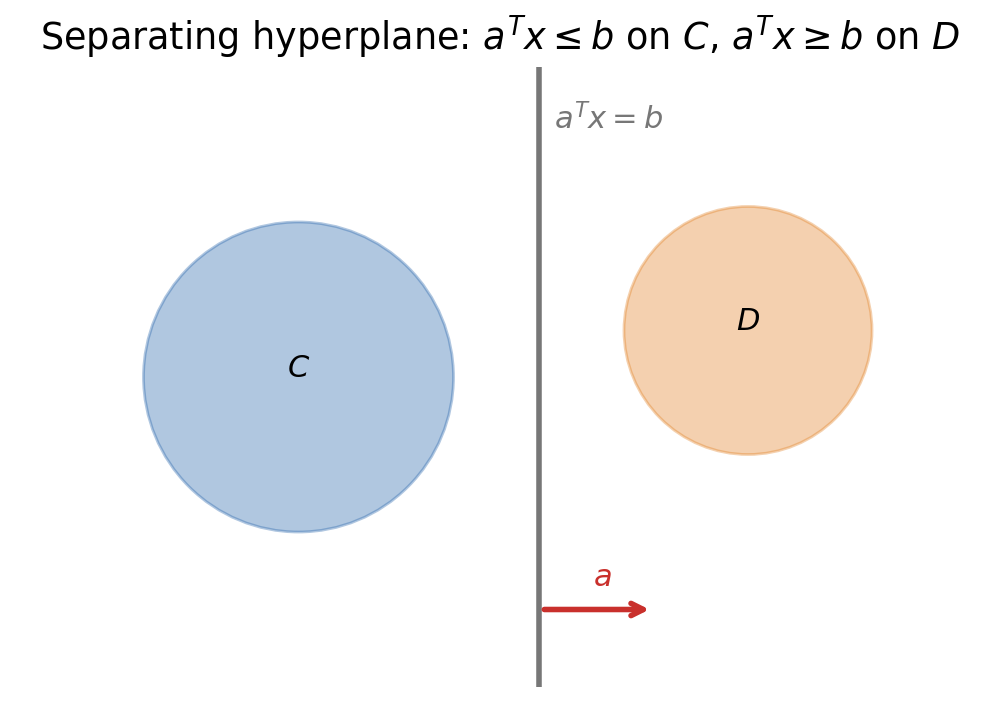
\includegraphics[width=.45\textwidth]{figures/separating_hyperplane.png}\end{figure}

\begin{pitfall}
Closedness of both sets is \emph{not} enough for strict separation. The standard counterexample (HW1 P2b, B\&V 2.23): $C_1=\{y\le0\}$ and $C_2=\{x>0,\ y\ge1/x\}$ in $\R^2$ are closed, convex, disjoint, but $\operatorname{dist}(C_1,C_2)=0$ because $(k,0)\in C_1$ and $(k,1/k)\in C_2$ get arbitrarily close. Only the non-strict separator $y=0$ exists. The underlying reason: two closed sets can have zero distance without intersecting when neither is bounded.
\end{pitfall}

\begin{figure}[H]\centering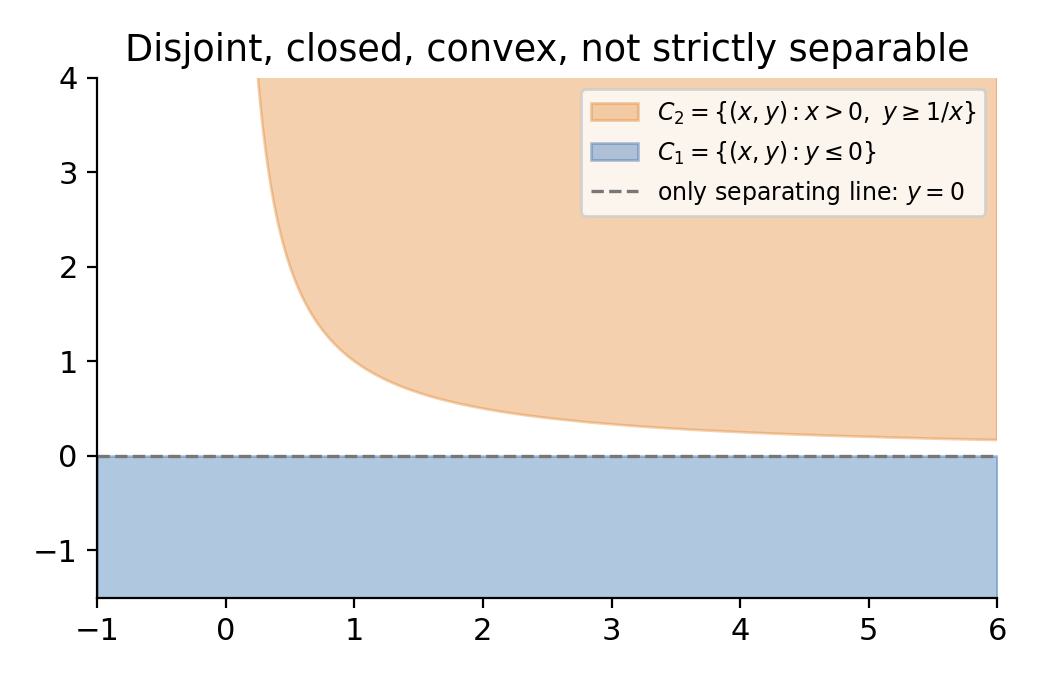
\includegraphics[width=.5\textwidth]{figures/no_strict_separation.png}\end{figure}

\begin{theorem}[Supporting hyperplane theorem]
If $C$ is convex and $x_0$ is a boundary point of $C$, there is $a\ne0$ with $a\T x\le a\T x_0$ for all $x\in C$. Conversely, a closed set with nonempty interior that has a supporting hyperplane at every boundary point is convex.
\end{theorem}
Proof sketch of the strict version, useful to remember: minimise $\|c-d\|$ over $c\in C,d\in D$ (a minimiser exists by compactness), and take the hyperplane through the midpoint of the minimising pair, normal $d-c$. The obstruction in the counterexample above is exactly that this minimum is not attained.

\section{Convex functions}

\subsection{Definition and the epigraph}
\begin{definition}[Convex function]
$f:\R^n\to\R$ (more generally, $f$ with convex domain $\dom f$) is \emph{convex} if for all $x,y\in\dom f$ and $\lam\in[0,1]$,
\[
f(\lam x+(1-\lam)y)\le\lam f(x)+(1-\lam)f(y).
\]
It is \emph{strictly convex} if the inequality is strict whenever $x\ne y$ and $\lam\in(0,1)$; \emph{concave} if $-f$ is convex.
\end{definition}
Geometrically: the chord between any two points on the graph lies \emph{on or above} the graph.

\begin{definition}[Epigraph and sublevel sets]
$\epi f=\{(x,t)\in\R^{n+1}: t\ge f(x)\}$ is the region above the graph. The $c$-sublevel set is $L_c=\{x: f(x)\le c\}$.
\end{definition}

\begin{theorem}
$f$ is convex $\iff$ $\epi f$ is a convex set.
\end{theorem}
This is the bridge between the ``sets'' and ``functions'' halves of the theory: every set result becomes a function result by applying it to epigraphs.

\begin{figure}[H]\centering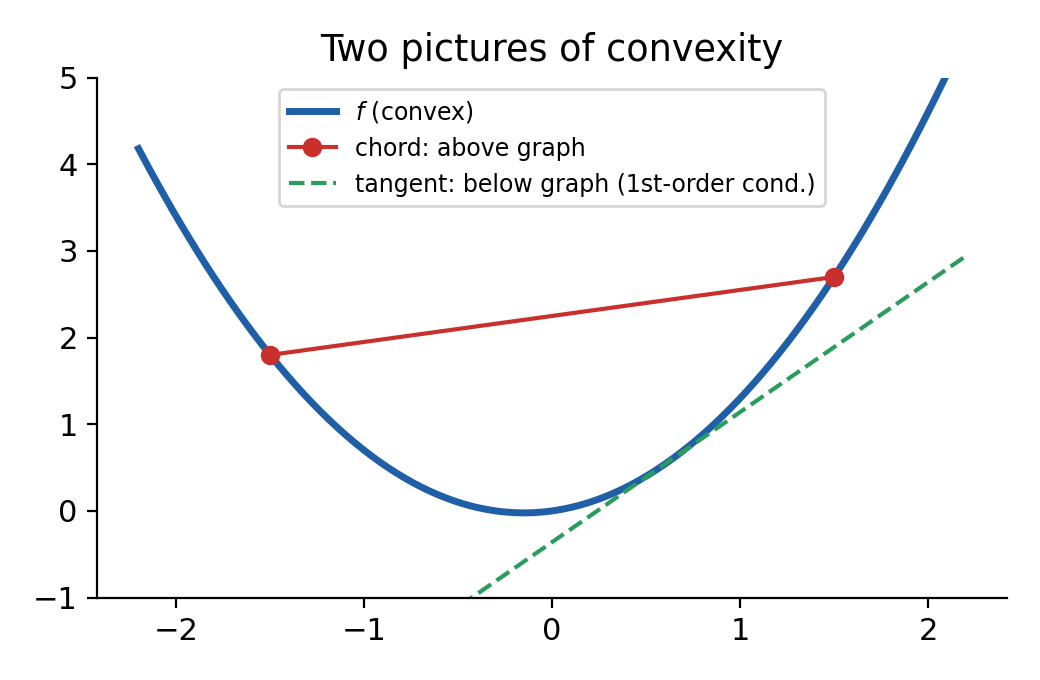
\includegraphics[width=.55\textwidth]{figures/convex_function.png}\end{figure}

\subsection{Tests for convexity}
\begin{theorem}[Restriction to lines]
$f$ is convex iff for every $x\in\dom f$ and direction $v$, the univariate function $g(t)=f(x+tv)$ is convex on $\{t:x+tv\in\dom f\}$.
\end{theorem}
\begin{theorem}[First-order condition]
If $f$ is differentiable with convex domain, $f$ is convex iff $\;f(y)\ge f(x)+\nabla f(x)\T(y-x)$ for all $x,y$. (Tangent planes lie below the graph; the linearisation is a \emph{global} underestimator.)
\end{theorem}
\begin{theorem}[Second-order condition]
If $f$ is twice differentiable with convex domain, $f$ is convex iff $\nabla^2f(x)\succeq0$ for all $x\in\dom f$. In one variable: $f''\ge0$. If $\nabla^2 f\succ0$ everywhere then $f$ is strictly convex (the converse fails: $x^4$).
\end{theorem}

\subsection{Examples}
\begin{center}\begin{tabular}{@{}ll@{}}\toprule
Convex & Concave \\ \midrule
$e^{ax}$ ($a\in\R$); $x^p$ on $x>0$ for $p\ge1$ or $p\le0$; $|x|^p$, $p\ge1$ & $\log x$; $x^p$ on $x>0$, $0\le p\le1$ \\
every norm $\|x\|$; $\max_i x_i$; $\log\sum_ie^{x_i}$ & geometric mean $(\prod x_i)^{1/n}$ on $\R^n_{++}$ \\
$x\T Px$ with $P\succeq0$; $a\T x+b$ (both) & $\log\det X$ on $\mathbb S^n_{++}$ \\
$x^2/y$ on $y>0$; $-\log x$ & $\min_i x_i$; entropy $-x\log x$ on $x>0$ \\ \bottomrule
\end{tabular}\end{center}

\subsection{Operations that preserve convexity of functions}
\begin{theorem}[Calculus of convex functions]
Let $f,f_1,\dots,f_k$ be convex.
\begin{enumerate}
\item \textbf{Nonnegative weighted sums.} $\sum_iw_if_i$ with $w_i\ge0$ is convex.
\item \textbf{Composition with affine map.} $g(x)=f(Ax+b)$ is convex.
\item \textbf{Pointwise maximum / supremum.} $\max\{f_1,\dots,f_k\}$ and $\sup_{\alpha}f_\alpha$ are convex. \emph{(HW1 P1c.)}
\item \textbf{Composition rules.} $h\circ g$ is convex if $h$ convex nondecreasing and $g$ convex; or $h$ convex nonincreasing and $g$ concave (with $\tilde h$ the extended-value extension).
\item \textbf{Partial minimisation.} If $f(x,y)$ is jointly convex and $C$ convex, $g(x)=\inf_{y\in C}f(x,y)$ is convex.
\item \textbf{Perspective.} $g(x,t)=t\,f(x/t)$ on $t>0$ is convex.
\end{enumerate}
\end{theorem}

\begin{proof}[Proof of 3 (the HW1 argument)]
Let $z=\lam x+(1-\lam)y$. For each $i$: $f_i(z)\le\lam f_i(x)+(1-\lam)f_i(y)\le\lam f_{\max}(x)+(1-\lam)f_{\max}(y)$. Take the max over $i$ on the left.
Equivalently: $\epi f_{\max}=\bigcap_i\epi f_i$, an intersection of convex sets.
\end{proof}

\begin{pitfall}
\textbf{Not preserved:} pointwise \textbf{minimum} ($\min\{x^2,(x-2)^2\}$ has a bump; $\epi f_{\min}=\bigcup\epi f_i$ is a union), \textbf{products} ($x\cdot x=x^2$ fine, but $x\cdot(-x)=-x^2$ is not), \textbf{differences} ($f_1-f_2$ is a difference of convex functions, ``DC,'' generally non-convex), and \textbf{arbitrary compositions} ($e^{-x}$ is convex, $-x^2$ concave, but $e^{-x^2}$ is neither). \emph{(HW1 P2a.)}
\end{pitfall}

\section{Sublevel sets and quasiconvexity}

\begin{proposition}[HW1 P2c]
If $f$ is convex, every sublevel set $L_c=\{x:f(x)\le c\}$ is convex.
\end{proposition}
\begin{proof}
$x,y\in L_c\Rightarrow f(\lam x+(1-\lam)y)\le\lam f(x)+(1-\lam)f(y)\le\lam c+(1-\lam)c=c$.
\end{proof}

\begin{pitfall}
\textbf{The converse is false.} Convex sublevel sets do \emph{not} imply a convex function. Counterexamples in one variable: $f(x)=\sqrt{|x|}$ (sublevel sets $[-c^2,c^2]$; but $f(2)=\sqrt2>1=\tfrac12f(0)+\tfrac12f(4)$), $f(x)=x^3$, $f(x)=-e^{-x^2}$, and indeed \emph{any monotone} function. In one variable, ``all sublevel sets convex'' just means ``all sublevel sets are intervals,'' which is far weaker than convexity.
\end{pitfall}

\begin{figure}[H]\centering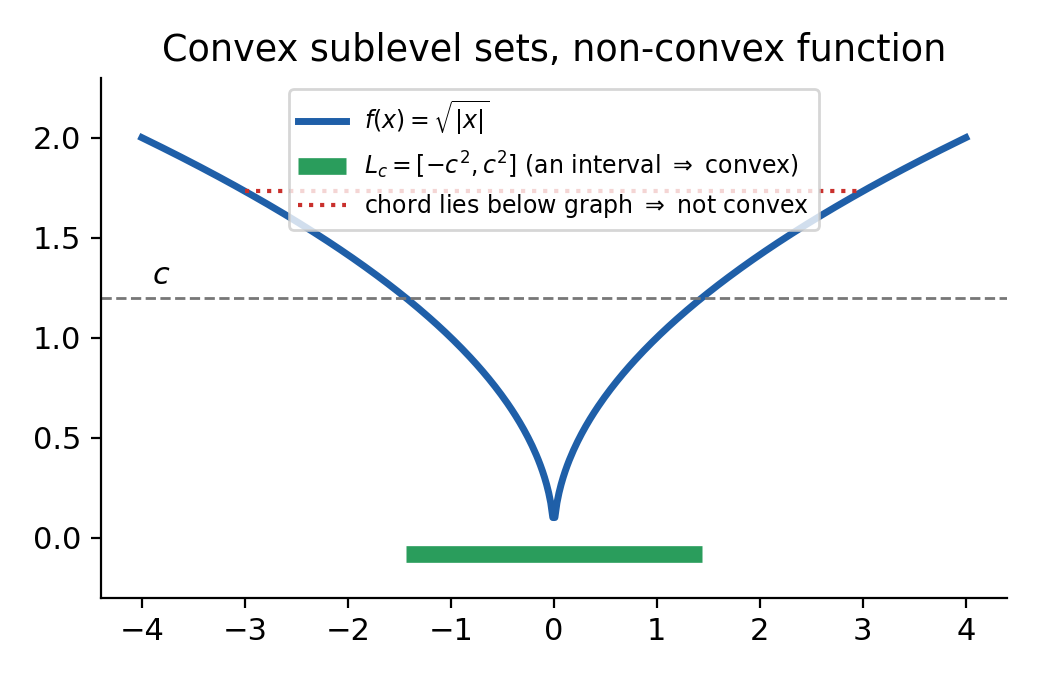
\includegraphics[width=.55\textwidth]{figures/quasiconvex.png}\end{figure}

\begin{definition}[Quasiconvex]
$f$ is \emph{quasiconvex} if every sublevel set is convex; equivalently $f(\lam x+(1-\lam)y)\le\max\{f(x),f(y)\}$.
\end{definition}
Hierarchy: \ convex $\Rightarrow$ quasiconvex, and the implication is strict. Quasiconvex problems can still be solved (by bisection on $c$ plus a convex feasibility problem for each $L_c$), which is why sublevel sets matter beyond this homework.

\begin{keyidea}
The right mental picture of ``$f$ convex $\Rightarrow$ $L_c$ convex'': slice the convex epigraph with the horizontal hyperplane $t=c$ and project down. Slicing (intersection with a convex set) and projecting (affine image) both preserve convexity. The converse fails because the sublevel sets are only \emph{horizontal} slices; convexity of $\epi f$ needs every slice, in every direction.
\end{keyidea}

\section{Proof toolkit}

\begin{template}
\emph{Set $C$ is convex (from the definition).}
\begin{enumerate}
\item ``Let $x,y\in C$ and $\lam\in[0,1]$. Set $z=\lam x+(1-\lam)y$.''
\item Unpack what $x\in C$ and $y\in C$ mean (an inequality, an equation, membership in other sets).
\item Show $z$ satisfies the same condition, using: linearity ($a\T z=\lam a\T x+(1-\lam)a\T y$), the triangle inequality plus homogeneity for norms ($\|\lam u+(1-\lam)v\|\le\lam\|u\|+(1-\lam)\|v\|$), or convexity of ingredient functions.
\item ``Hence $z\in C$, so $C$ is convex.''
\end{enumerate}
\end{template}

\begin{template}
\emph{Function $f$ is convex (from the definition).} Same skeleton; the target inequality is $f(z)\le\lam f(x)+(1-\lam)f(y)$. Chain inequalities: apply convexity of the pieces first, then bound each piece by something involving $f(x),f(y)$, keeping the weights $\lam,1-\lam\ge0$ in front.
\end{template}

\begin{template}
\emph{Something is NOT convex.} One explicit witness suffices: specific $x,y,\lam$ (usually $\lam=\tfrac12$ and small integers) for which the defining condition fails. Compute both sides numerically and state the strict inequality. Draw the picture to find the witness: look for a ``bump'' (functions) or a ``notch/gap'' (sets).
\end{template}

\begin{template}
\emph{Geometric $\to$ algebraic (``show this region is a half-space'').} Write the geometric condition as an inequality, square if both sides are nonnegative, expand, cancel the nonlinear terms, and read off $c$ and $d$. Verify with two test points.
\end{template}

\begin{template}
\emph{No strict separation exists.} Assume $a\T p<b<a\T q$ for all $p\in C$, $q\in D$. Send points of $C$ to infinity in various directions to force components of $a$ to vanish or have a sign; then find a sequence in $D$ whose $a\T q$ tends to a value $\le b$. Contradiction.
\end{template}

\section{Self-test questions}
Try these without looking back; short answers follow.

\begin{exercise}
Is $\{x\in\R^n: \|x\|_2\le1\}\cap\{x: x_1\ge0\}$ convex? Is $\{x:\|x\|_2\le1\}\cup\{x:\|x-3e_1\|_2\le1\}$?
\end{exercise}
\begin{exercise}
Is $f(x)=\max\{|x_1|,\,x_2^2,\,e^{x_3}\}$ convex on $\R^3$? Is $g(x)=\min\{|x|,1\}$ convex on $\R$?
\end{exercise}
\begin{exercise}
Write $\{x:\|x-v_1\|\le\|x-v_2\|\}$ for $v_1=(0,0)$, $v_2=(2,2)$ in the form $c\T x\le d$.
\end{exercise}
\begin{exercise}
Give a convex function on $\R$ that is not strictly convex, and a strictly convex function whose second derivative vanishes somewhere.
\end{exercise}
\begin{exercise}
Is $\{x: \|Ax+b\|_2\ge c\T x+d\}$ convex in general? What about $\{x:\|Ax+b\|_2\le c\T x+d\}$?
\end{exercise}
\begin{exercise}
The half-space $\{x: 2x_1-x_2\le 4\}$ is contained in $\{x:\tilde a\T x\le\tilde b\}$. What can you say about $\tilde a$ and $\tilde b$?
\end{exercise}
\begin{exercise}
Distance between $\{x_1+2x_2+2x_3=1\}$ and $\{x_1+2x_2+2x_3=7\}$?
\end{exercise}
\begin{exercise}
True or false: if all sublevel sets of $f$ are convex and $f$ is differentiable, then $f$ is convex.
\end{exercise}

\subsection*{Answers}
\begin{enumerate}
\item Yes (intersection of a ball and a half-space). No: $e_1$ and $2e_1$ are in the union but $1.5e_1$ is not.
\item Yes: max of convex functions (each is convex: a norm, a convex quadratic, an exponential). No: $g(0)=0,\ g(2)=1,\ g(1)=1>\tfrac12(0+1)$; it flattens out, a pointwise min of convex functions.
\item $c=2(v_2-v_1)=(4,4)$, $d=\|v_2\|^2-\|v_1\|^2=8$, i.e.\ $x_1+x_2\le2$. Check: $v_1=(0,0)$ satisfies it, $v_2=(2,2)$ does not.
\item $f(x)=|x|$ or any affine function (convex, not strictly); $f(x)=x^4$ (strictly convex, $f''(0)=0$).
\item The ``$\ge$'' set is generally not convex (it is the complement of a convex set's interior, e.g.\ $\{|x|\ge1\}$). The ``$\le$'' set is convex: preimage of the second-order cone under an affine map.
\item $\tilde a=\lam(2,-1)$ and $\tilde b\ge4\lam$ for some $\lam>0$.
\item $|1-7|/\|(1,2,2)\|=6/3=2$.
\item False: $f(x)=x^3$ is smooth with sublevel sets $(-\infty,c^{1/3}]$, but $f''(x)<0$ for $x<0$.
\end{enumerate}

\section{One-page cheat sheet}
\begin{center}\renewcommand{\arraystretch}{1.25}
\begin{tabular}{@{}>{\raggedright}p{.32\textwidth}p{.6\textwidth}@{}}\toprule
Convex set & $x,y\in C,\ \lam\in[0,1]\Rightarrow\lam x+(1-\lam)y\in C$ \\
Convex function & $f(\lam x+(1-\lam)y)\le\lam f(x)+(1-\lam)f(y)$; equivalently $\epi f$ convex \\
1st-order test & $f(y)\ge f(x)+\nabla f(x)\T(y-x)$ \\
2nd-order test & $\nabla^2f\succeq0$ \\
Sets: preserved by & intersection (any family), affine image/preimage, sums, products, perspective \\
Sets: NOT preserved by & union, complement \\
Functions: preserved by & nonneg.\ sums, affine composition, pointwise max/sup, monotone convex composition, partial inf, perspective \\
Functions: NOT preserved by & pointwise min, products, differences, general composition \\
Sublevel sets & convex $f\Rightarrow$ $L_c$ convex; converse false ($\sqrt{|x|}$, $x^3$); ``all $L_c$ convex'' $=$ quasiconvex \\
Hyperplane / half-space & $\{a\T x=b\}$ / $\{a\T x\le b\}$, normal $a$ points to the $\ge$ side \\
Point--plane distance & $|a\T x-b|/\|a\|_2$ \\
Parallel planes distance & $|b_1-b_2|/\|a\|_2$ \\
Half-space containment & $\{a\T x\le b\}\subseteq\{\tilde a\T x\le\tilde b\}\iff\tilde a=\lam a,\ \tilde b\ge\lam b,\ \lam>0$ \\
Closer to $v_1$ than $v_2$ & $2(v_2-v_1)\T x\le\|v_2\|^2-\|v_1\|^2$ (perpendicular bisector) \\
Separation & disjoint convex $\Rightarrow$ separating hyperplane; strict needs closed + compact \\
Strict-separation counterexample & $\{y\le0\}$ vs.\ $\{x>0,\ y\ge1/x\}$: closed, disjoint, distance $0$ \\
Second-order cone set & $\{x:\|Ax+b\|_2\le c\T x+d\}$ convex (affine preimage of $\{\|u\|\le t\}$) \\ \bottomrule
\end{tabular}\end{center}

\bigskip\noindent\textbf{Further reading.} Boyd \& Vandenberghe, \emph{Convex Optimization}, Chapter~2 (sets, \S2.1--2.5) and Chapter~3 (functions, \S3.1--3.4). Exercises 2.1--2.12, 2.23, 3.1--3.10 are the best drill for this material.

\end{document}
